% Informe técnico Rejas-GNN v0.3 — compilar con XeLaTeX (dos pasadas)
\documentclass[11pt,a4paper]{article}

\usepackage{fontspec}
\usepackage{polyglossia}
\setmainlanguage{spanish}
\gappto\captionsspanish{\renewcommand{\tablename}{Tabla}}
\setmainfont{TeX Gyre Pagella}
\setmonofont{DejaVu Sans Mono}[Scale=0.85]
\usepackage{unicode-math}
\setmathfont{Latin Modern Math}
\setmathfont{TeX Gyre Pagella}[range={up/num,up/Latin,up/latin,it/Latin,it/latin}]

\usepackage[margin=2.5cm]{geometry}
\usepackage{microtype}
\usepackage{graphicx}
\usepackage{booktabs}
\usepackage{tabularx}
\usepackage{array}
\usepackage{caption}
\usepackage{enumitem}
\usepackage{xcolor}
\usepackage{float}
\usepackage[hidelinks]{hyperref}

\definecolor{acento}{HTML}{8B1E1E}
\captionsetup{font=small,labelfont=bf,format=hang}
\setlist{itemsep=2pt,topsep=4pt}
\newcolumntype{Y}{>{\raggedright\arraybackslash}X}
\newcommand{\codigo}[1]{\texttt{#1}}

\hypersetup{
  pdftitle={¿Qué calles se cierran? Predicción de cierres residenciales en Pedro Aguirre Cerda},
  pdfauthor={Gerardo Ramos}
}

\title{\textbf{¿Qué calles se cierran?}\\[4pt]
\large Predicción de cierres residenciales en Pedro Aguirre Cerda\\
a partir de la morfología de la red vial, con validación espacial}
\author{Gerardo Ramos}
\date{Informe técnico · Versión 0.3.0 · Noviembre de 2026\\[2pt]
\small Repositorio: \url{https://github.com/gdosramos/rejas-gnn}}

\begin{document}
\maketitle

\begin{abstract}
\noindent En la comuna de Pedro Aguirre Cerda (Santiago de Chile), los vecinos han cerrado con rejas y
portones cientos de pasajes y calles. Un levantamiento clasificó los 2\,790 tramos viales de la
comuna, de los cuales 217 (7,8\,\%) tienen un cierre social. Este trabajo convierte una pregunta
descriptiva en una falsable: ¿puede un modelo que nunca vio un barrio predecir cuáles de sus tramos
están cerrados? Para impedir que un modelo obtenga buenos puntajes copiando la etiqueta del pasaje
vecino, la evaluación usa validación cruzada por bloques espaciales con zonas de amortiguación de
200\,m. Se comparan dos modelos no neuronales (una tabla de dos variables y una regresión
logística), un perceptrón multicapa y tres redes neuronales de grafos (GCN, GraphSAGE y GATv2),
con y sin covariables socioeconómicas zonales, y cada afirmación se contrasta con diferencias
pareadas sobre las mismas particiones. Los resultados muestran que los cierres son predecibles en
barrios no vistos (ROC-AUC 0,87; PR-AUC 0,29, es decir, 3,7 veces el azar), pero que el mejor
modelo es lineal, que la señal se concentra en pocas variables (clase de vía, pasaje sin salida y
posición en la comuna), que el grafo no agrega información demostrable y que las covariables
socioeconómicas no mejoran la predicción. Los cierres se registraron en dos cohortes que siguen a
las dos leyes que regulan los cierres en Chile; un modelo entrenado solo con la primera predice la
segunda tan bien como uno entrenado con ella, lo que descarta que el modelo aprenda únicamente la
elegibilidad legal del primer régimen.
\end{abstract}

\section{La pregunta}

En Pedro Aguirre Cerda (PAC), una comuna popular de Santiago, los residentes han enrejado una
fracción considerable de sus pasajes, práctica conocida localmente como \emph{rejas}. El patrón es
visible en un mapa; lo que no es evidente es si es \emph{predecible}. La pregunta de este trabajo es:

\begin{quote}
\emph{¿Se puede predecir qué tramos viales se cierran a partir de su posición en la red vial y de
las características de su entorno, y cuánto aporta cada tipo de información?}
\end{quote}

Un trabajo exploratorio previo, no publicado, sobre los mismos datos describió el patrón con dos herramientas exploratorias: un
campo de densidad fractal y un mapa autoorganizado (SOM) sobre índices de bienestar territorial.
Este trabajo reformula la pregunta como una afirmación falsable: un modelo que nunca vio un barrio
debe predecir sus cierres, y se mide cuán bien lo hace. El diseño es predictivo; no permite
afirmaciones causales sobre por qué los vecinos cierran sus calles.

\section{Los datos}

Los cierres no están dispersos. Aparecen en \emph{peinetas}: filas de pasajes cortos, paralelos y
sin salida que desembocan en una calle colectora, la morfología típica de los conjuntos de vivienda
social construidos entre las décadas de 1960 y 1980. El pasaje es la unidad que se cierra y, como
los pasajes vienen en series, también los cierres (figura~\ref{fig:red}).

\begin{figure}[H]
  \centering
  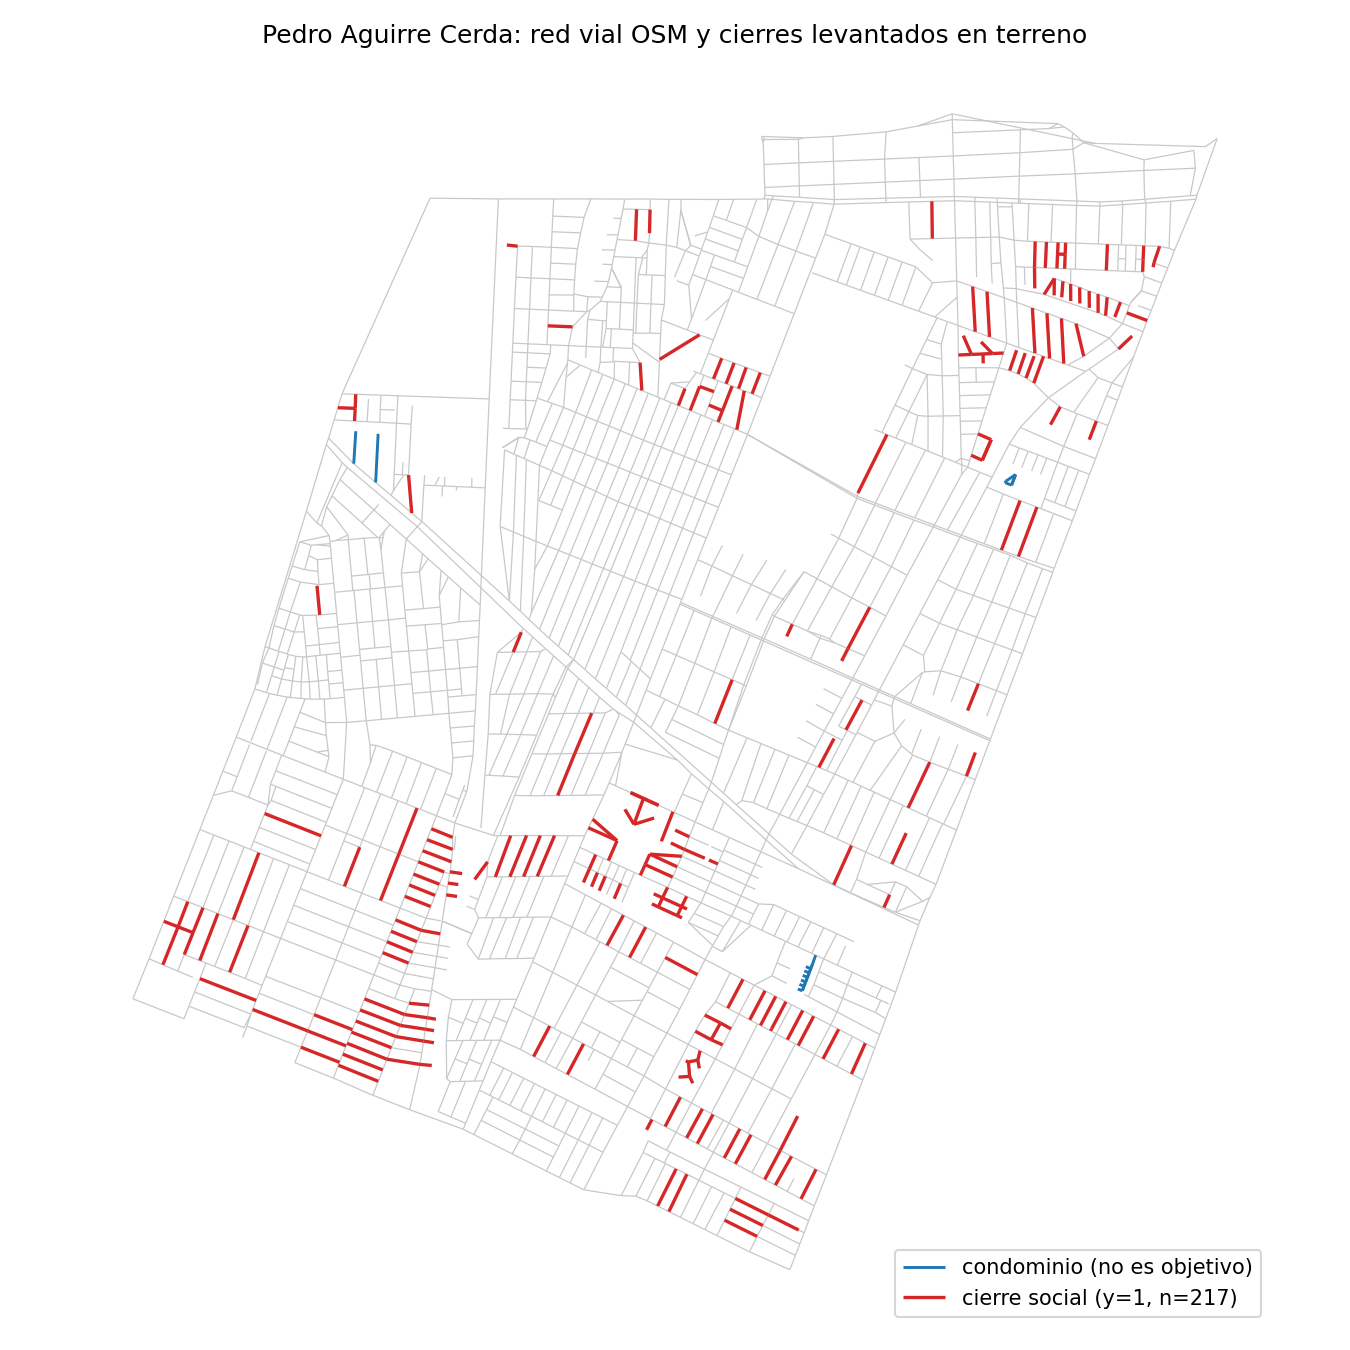
\includegraphics[width=0.62\textwidth]{../figures/fig01a_red_y_cierres.png}
  \caption{Red vial de PAC. En rojo, los cierres sociales; en azul, los portones de condominios.}
  \label{fig:red}
\end{figure}

\begin{table}[H]
  \centering
  \caption{Resumen de los datos.}
  \label{tab:datos}
  \begin{tabular}{lr}
    \toprule
    Tramos viales (aristas de OpenStreetMap) & 2\,790 \\
    Cierres sociales (\codigo{cierre} + \codigo{informal} + \codigo{medio}), la etiqueta & \textbf{217 (7,8\,\%)} \\
    Portones de condominio (estructurales, no son etiqueta) & 22 \\
    Intersecciones & 1\,826 \\
    Autocorrelación espacial de la etiqueta (I de Moran en el grafo dual) & 0,17 \\
    \bottomrule
  \end{tabular}
\end{table}

Las variables morfológicas más simples ya son muy informativas (figura~\ref{fig:tasas}). Las
calles de convivencia (\codigo{living\_street}), las vías de servicio y las peatonales se cierran
entre el 18 y el 23\,\% de las veces; las calles residenciales, el 1,5\,\%; las avenidas, nunca.
Un tramo sin salida se cierra 5,7 veces más a menudo que uno con salida (35,5\,\% frente a 6,2\,\%).

\begin{figure}[H]
  \centering
  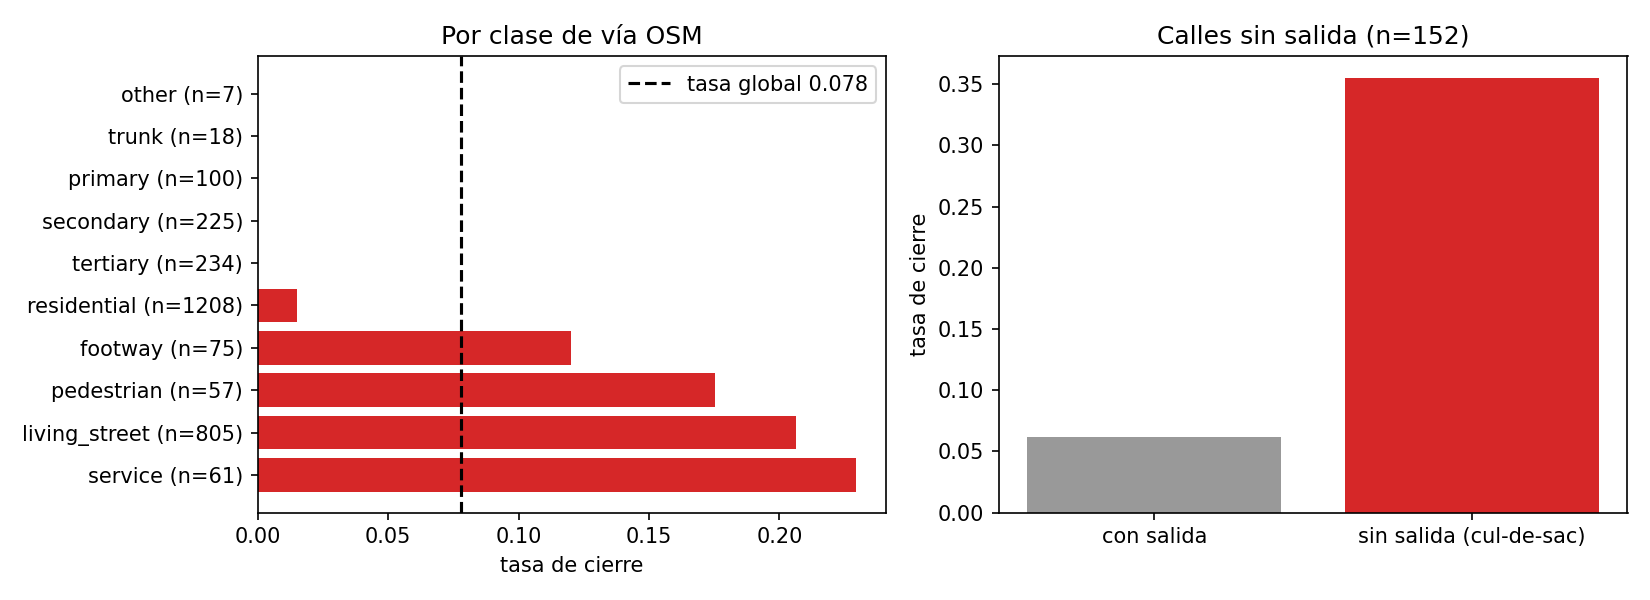
\includegraphics[width=\textwidth]{../figures/fig01c_tasa_por_tipo.png}
  \caption{Tasa de cierre por clase de vía OSM (izquierda) y según si el tramo es sin salida
  (derecha). La línea punteada marca la tasa global.}
  \label{fig:tasas}
\end{figure}

\paragraph{Dos cohortes de registro.} La columna \codigo{año} indica el año en que se registró
el cierre; los tramos abiertos llevan el año del levantamiento (2025). Los cierres se concentran en
dos cohortes: 109 en 2012--2015 y 108 en 2022--2025. Ambas cohortes siguen a las dos leyes que regulan los cierres en Chile. La
Ley 20.499 (2011) permitió cerrar calles y pasajes por motivos de seguridad con la condición de que
tuvieran una misma vía de acceso y salida~\cite{ley20499}; la Ley 21.411 (2022) extendió la
posibilidad a calles con acceso y salida distintos, con calzada de menos de siete metros y una
extensión no superior a una cuadra~\cite{ley21411}. Los datos son consistentes con esa secuencia:
el 31\,\% de los cierres de 2012--2015 son tramos sin salida, frente al 19\,\% de los de
2022--2025. Esto plantea una hipótesis alternativa, que el modelo aprenda la elegibilidad legal y
no el comportamiento de los vecinos, que se pone a prueba en la sección~\ref{sec:resultados}.

\section{Qué ve el modelo}

El objeto natural para una pregunta a nivel de tramo es el \textbf{grafo dual} (\emph{line graph})
de la red vial: cada tramo es un nodo y dos tramos son vecinos si comparten una intersección. Sobre
este grafo la tarea es de clasificación de nodos, y las redes neuronales de grafos pueden, en
principio, aprovechar lo que ocurre en los tramos vecinos~\cite{kipf2017,hamilton2017,brody2022}.

Cada tramo se describe con dos bloques de atributos, y el contraste entre ellos es la ablación
central del estudio (tabla~\ref{tab:bloques}).

\begin{table}[H]
  \centering
  \caption{Bloques de atributos.}
  \label{tab:bloques}
  \begin{tabularx}{\textwidth}{lYr}
    \toprule
    Bloque & Contenido & N.º \\
    \midrule
    A · Topología y geometría & Grado, intermediación, cercanía, agrupamiento, puente, punto de
      articulación, \textbf{sin salida}; largo, orientación, distancia al centroide de la comuna,
      clase de vía OSM & 28 \\
    B · A + socioeconómicas zonales & A más 50 variables del Censo 2024 y 21 de la Matriz de
      Bienestar Humano Territorial 2017 (cada fuente incluye el número de manzanas promediadas),
      asignadas desde las manzanas a menos de 150\,m, más 2 indicadores de datos faltantes & 101 \\
    \bottomrule
  \end{tabularx}
\end{table}

Las covariables del bloque~B se asignan a cada tramo como el promedio, ponderado por el inverso de
la distancia, de las manzanas cuyo centroide está a menos de 150\,m. El resultado es un campo
suave: tramos vecinos reciben valores casi idénticos. Siete tramos tienen datos faltantes; se
imputan por la mediana y se marcan con un indicador por fuente. En la versión anterior se agregaba
un indicador por columna, lo que producía 69 columnas casi idénticas y un bloque de 168 variables;
la ablación se repitió sin ellas.

Este bloque tiene tres limitaciones conocidas. Su \textbf{temporalidad no coincide con la
etiqueta}: para la mayoría de los cierres, el Censo 2024 e incluso la MBHT 2017 se midieron
\emph{después} de instalado el portón. Es \textbf{zonal}: describe la manzana, no el pasaje. Y en
los índices de seguridad existe una posible \textbf{causalidad inversa}: un pasaje enrejado puede
modificar el delito registrado.

\section{La trampa: una partición aleatoria sería hacer trampa}

Como los cierres vienen en peinetas, un pasaje de prueba elegido al azar casi siempre tiene a sus
hermanos (misma peineta, misma etiqueta) en el conjunto de entrenamiento, a 30\,m de distancia.
Cualquier modelo, y más aún una red de grafos, puntuaría alto copiando al vecino, sin aprender nada
transferible a un barrio no levantado.

Por eso la evaluación usa \textbf{validación cruzada por bloques espaciales con zonas de
amortiguación}~\cite{roberts2017}. La comuna se divide en 20 bloques contiguos (k-medias sobre
coordenadas métricas); en cada uno de los 5 pliegues, algunos bloques forman el conjunto de prueba,
un cuarto de los restantes se usa para la detención temprana y la elección de umbrales, y todo tramo
a menos de 200\,m de un tramo de prueba pierde su etiqueta (permanece en el grafo, pero no enseña
nada).

\begin{figure}[H]
  \centering
  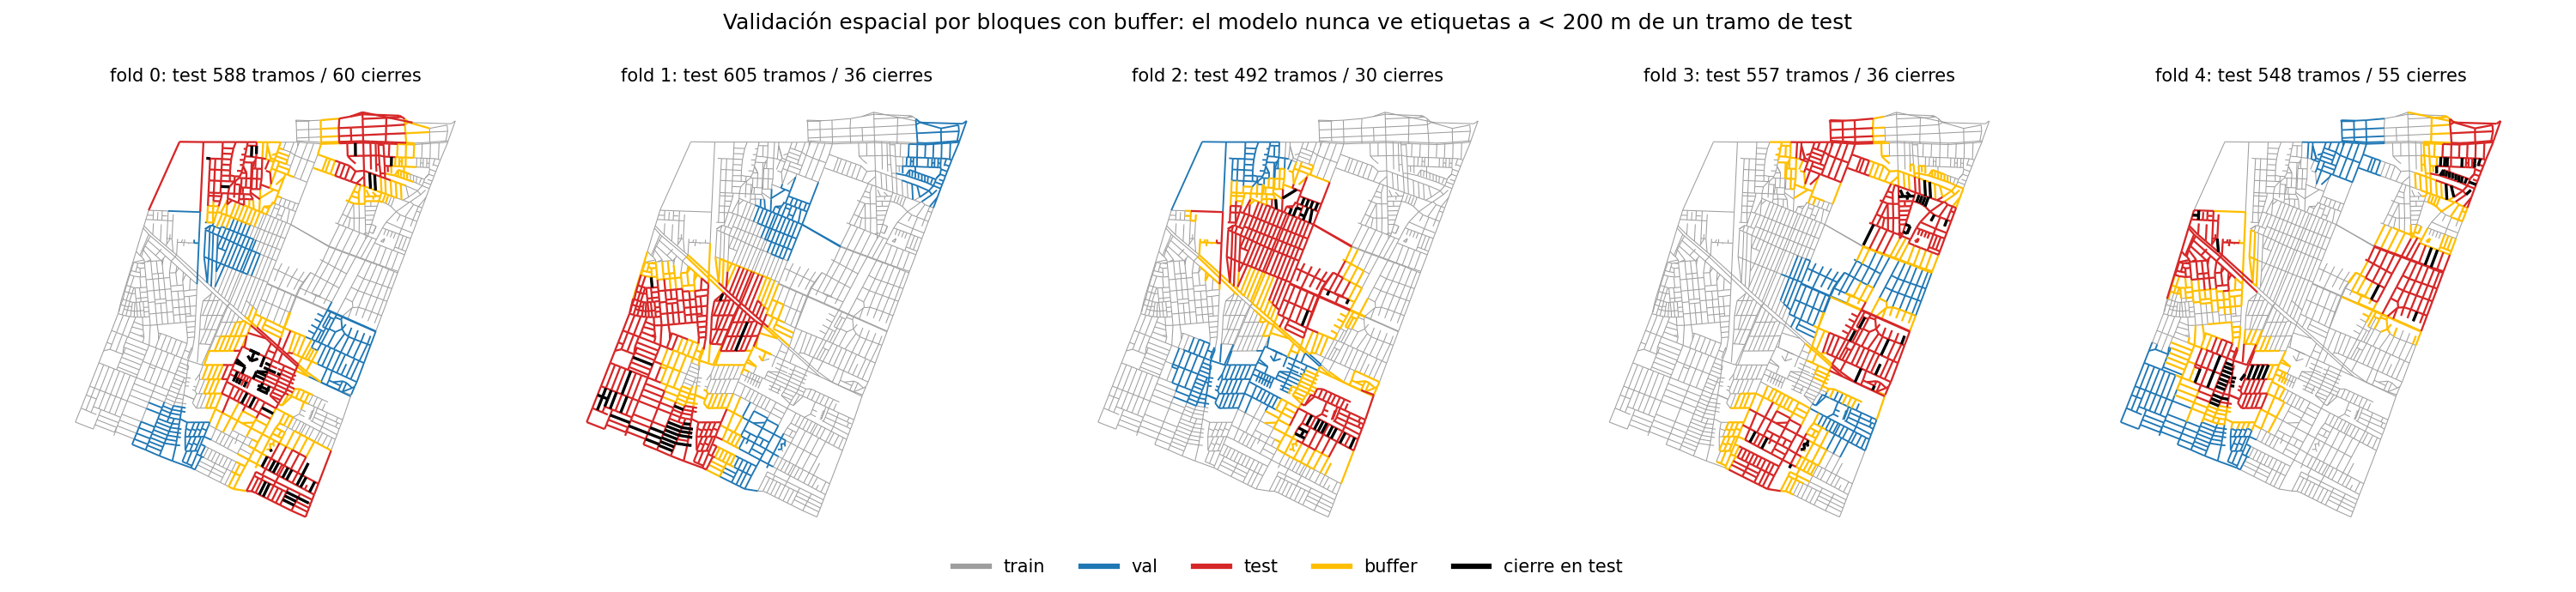
\includegraphics[width=\textwidth]{../figures/fig02b_folds.png}\\[4pt]
  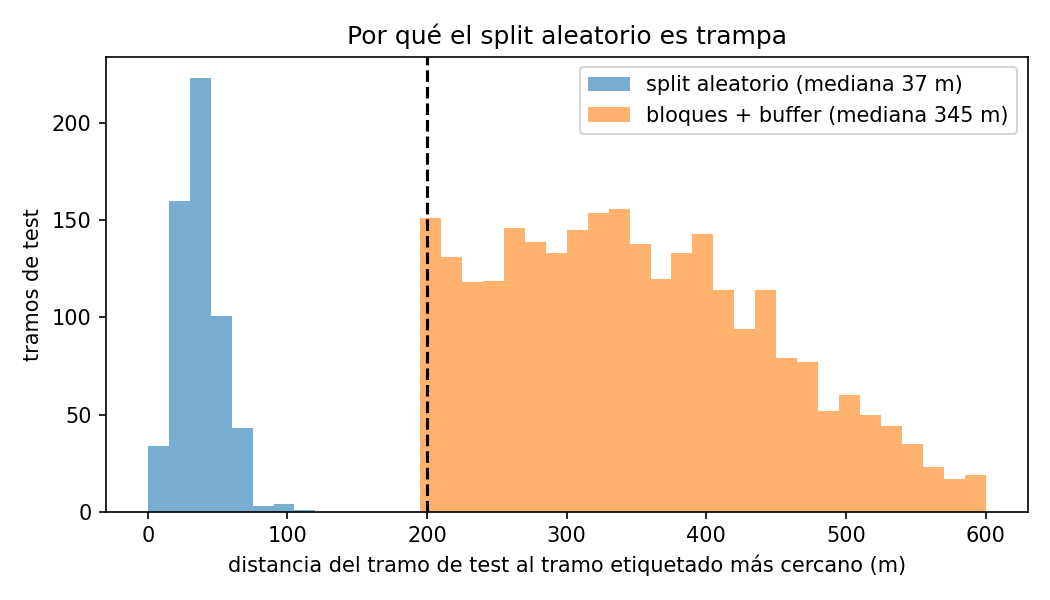
\includegraphics[width=0.6\textwidth]{../figures/fig02c_distancia_fuga.png}
  \caption{Arriba: los cinco pliegues espaciales (prueba en rojo, amortiguación en amarillo,
  validación en azul, entrenamiento en gris). Abajo: distancia de cada tramo de prueba al tramo
  etiquetado más cercano, con partición aleatoria y con bloques y amortiguación.}
  \label{fig:folds}
\end{figure}

Con una partición aleatoria, el 99\,\% de los tramos de prueba tiene un tramo etiquetado a menos
de 100\,m; con bloques y amortiguación, ninguno a menos de 200\,m. El precio es real y está
declarado: cada pliegue entrena con solo 83 a 136 de los 217 cierres, y la estimación es
deliberadamente pesimista, porque mide extrapolación a un barrio nuevo, que es lo que la pregunta
pide.

\section{El experimento}

\begin{itemize}
  \item \textbf{Modelos.} Dos líneas base no neuronales: una tabla de consulta con 12 celdas,
    \[ P(\text{cierre}\mid\text{clase de vía},\ \text{sin salida}), \]
    y una regresión
    logística con regularización L2. Un perceptrón multicapa (MLP) que ignora el grafo y tres redes
    de grafos que lo usan: GCN~\cite{kipf2017}, GraphSAGE~\cite{hamilton2017} y
    GATv2~\cite{brody2022}, implementadas con PyTorch Geometric~\cite{fey2019}.
  \item \textbf{Ablación.} Cada modelo neuronal se entrena dos veces: con el bloque~A y con A+B.
    La regresión logística se reajusta además sin la clase de vía y sin la distancia al centroide,
    para identificar el origen de su señal.
  \item \textbf{Repetición.} Diez semillas (42--51). La semilla fija la partición en bloques, de
    modo que en cada semilla todos los modelos se evalúan sobre exactamente los mismos barrios
    retenidos.
  \item \textbf{Optimización de los modelos neuronales.} Entropía cruzada binaria ponderada (los
    positivos son 1 de cada 12), Adam y detención temprana por PR-AUC de validación. Todas las
    arquitecturas comparten los mismos hiperparámetros; no hubo ajuste específico por arquitectura.
  \item \textbf{Métricas.} Para el ordenamiento, PR-AUC (la métrica honesta con 7,8\,\% de
    positivos; el azar vale 0,078)~\cite{saito2015} y ROC-AUC. Para las probabilidades, el puntaje
    de Brier~\cite{brier1950}, el error de calibración esperado (ECE) y el \textbf{puntaje de
    habilidad de Brier} frente a predecir la prevalencia $\pi$ para todos los tramos:
    \begin{equation}
      \mathrm{BSS} = 1 - \frac{\frac{1}{N}\sum_{i}(p_i - y_i)^2}{\pi\,(1-\pi)} .
    \end{equation}
    Un BSS positivo indica que las probabilidades son más informativas que la tasa base; uno
    negativo, que no lo son. Las probabilidades se calibran con regresión isotónica ajustada solo
    sobre los bloques de validación.
  \item \textbf{Comparaciones.} Cada afirmación del tipo «A es mejor que B» se contrasta con las
    diez diferencias por semilla sobre las mismas particiones: diferencia media, intervalo de
    confianza del 95\,\% por \emph{bootstrap} y prueba exacta de rangos con signo de
    Wilcoxon~\cite{wilcoxon1945}. Con diez semillas, el menor valor $p$ alcanzable es 0,002, y una
    diferencia no significativa significa «no demostrada», no «igual».
\end{itemize}

\section{Resultados}
\label{sec:resultados}

La tabla~\ref{tab:resultados} resume el desempeño en los bloques de prueba con el bloque~A. Las
tablas completas, incluido el bloque A+B, están en el repositorio
(\codigo{docs/reference\_results/v03\_apple\_m1/}).

\begin{table}[H]
  \centering
  \caption{Desempeño en los bloques de prueba, media $\pm$ desviación estándar sobre diez semillas,
  atributos del bloque~A (ejecución en Apple M1).}
  \label{tab:resultados}
  \small
  \begin{tabular}{lcccc}
    \toprule
    Modelo & Atrib. & PR-AUC & ROC-AUC & BSS cal. \\
    \midrule
    \textbf{Regresión logística} & 28 & $\mathbf{0{,}286 \pm 0{,}024}$ & $\mathbf{0{,}871 \pm 0{,}012}$ & $\mathbf{+0{,}056}$ \\
    Logística sin distancia al centroide & 27 & $0{,}218 \pm 0{,}018$ & $0{,}822 \pm 0{,}016$ & $-0{,}002$ \\
    MLP & 28 & $0{,}211 \pm 0{,}023$ & $0{,}787 \pm 0{,}061$ & $-0{,}067$ \\
    GraphSAGE & 28 & $0{,}206 \pm 0{,}031$ & $0{,}755 \pm 0{,}048$ & $-0{,}080$ \\
    Tabla clase de vía $\times$ sin salida & 2 & $0{,}202 \pm 0{,}025$ & $0{,}805 \pm 0{,}018$ & $+0{,}011$ \\
    Logística sin clase de vía & 18 & $0{,}197 \pm 0{,}018$ & $0{,}772 \pm 0{,}013$ & $-0{,}003$ \\
    GATv2 & 28 & $0{,}127 \pm 0{,}022$ & $0{,}636 \pm 0{,}028$ & $-0{,}165$ \\
    GCN & 28 & $0{,}122 \pm 0{,}019$ & $0{,}611 \pm 0{,}050$ & $-0{,}116$ \\
    \bottomrule
  \end{tabular}
\end{table}

\begin{table}[H]
  \centering
  \caption{Diferencias pareadas A$-$B sobre las diez semillas, con intervalo de confianza del
  95\,\% por \emph{bootstrap}. Una diferencia se considera respaldada cuando su intervalo excluye
  el cero.}
  \label{tab:pareadas}
  \small
  \renewcommand{\arraystretch}{1.25}\begin{tabular}{@{}lccc@{}}
    \toprule
    Comparación & $\Delta$PR-AUC & $\Delta$ROC-AUC & $\Delta$BSS \\
    \midrule
    Regresión logística $-$ MLP & \begin{tabular}[t]{@{}c@{}}$+0{,}076$\\[-1pt]{\footnotesize$[+0{,}061;\ +0{,}092]$}\end{tabular} & \begin{tabular}[t]{@{}c@{}}$+0{,}084$\\[-1pt]{\footnotesize$[+0{,}053;\ +0{,}125]$}\end{tabular} & \begin{tabular}[t]{@{}c@{}}$+0{,}124$\\[-1pt]{\footnotesize$[+0{,}084;\ +0{,}172]$}\end{tabular} \\
    MLP $-$ GraphSAGE & \begin{tabular}[t]{@{}c@{}}$+0{,}005$\\[-1pt]{\footnotesize$[-0{,}018;\ +0{,}027]$}\end{tabular} & \begin{tabular}[t]{@{}c@{}}$+0{,}032$\\[-1pt]{\footnotesize$[-0{,}001;\ +0{,}064]$}\end{tabular} & \begin{tabular}[t]{@{}c@{}}$+0{,}013$\\[-1pt]{\footnotesize$[-0{,}031;\ +0{,}055]$}\end{tabular} \\
    MLP $-$ tabla de dos variables & \begin{tabular}[t]{@{}c@{}}$+0{,}009$\\[-1pt]{\footnotesize$[-0{,}002;\ +0{,}019]$}\end{tabular} & \begin{tabular}[t]{@{}c@{}}$-0{,}018$\\[-1pt]{\footnotesize$[-0{,}049;\ +0{,}006]$}\end{tabular} & \begin{tabular}[t]{@{}c@{}}$-0{,}078$\\[-1pt]{\footnotesize$[-0{,}142;\ -0{,}020]$}\end{tabular} \\
    Bloque A $-$ A+B, MLP & \begin{tabular}[t]{@{}c@{}}$+0{,}006$\\[-1pt]{\footnotesize$[-0{,}016;\ +0{,}030]$}\end{tabular} & \begin{tabular}[t]{@{}c@{}}$+0{,}050$\\[-1pt]{\footnotesize$[+0{,}008;\ +0{,}089]$}\end{tabular} & \begin{tabular}[t]{@{}c@{}}$+0{,}015$\\[-1pt]{\footnotesize$[-0{,}023;\ +0{,}059]$}\end{tabular} \\
    Bloque A $-$ A+B, GraphSAGE & \begin{tabular}[t]{@{}c@{}}$+0{,}025$\\[-1pt]{\footnotesize$[+0{,}004;\ +0{,}047]$}\end{tabular} & \begin{tabular}[t]{@{}c@{}}$+0{,}064$\\[-1pt]{\footnotesize$[+0{,}025;\ +0{,}094]$}\end{tabular} & \begin{tabular}[t]{@{}c@{}}$+0{,}046$\\[-1pt]{\footnotesize$[-0{,}023;\ +0{,}118]$}\end{tabular} \\
    GraphSAGE $-$ GCN & \begin{tabular}[t]{@{}c@{}}$+0{,}084$\\[-1pt]{\footnotesize$[+0{,}059;\ +0{,}107]$}\end{tabular} & \begin{tabular}[t]{@{}c@{}}$+0{,}144$\\[-1pt]{\footnotesize$[+0{,}112;\ +0{,}174]$}\end{tabular} & \begin{tabular}[t]{@{}c@{}}$+0{,}036$\\[-1pt]{\footnotesize$[-0{,}001;\ +0{,}072]$}\end{tabular} \\
    Logística: completa $-$ sin clase de vía & \begin{tabular}[t]{@{}c@{}}$+0{,}089$\\[-1pt]{\footnotesize$[+0{,}079;\ +0{,}100]$}\end{tabular} & \begin{tabular}[t]{@{}c@{}}$+0{,}099$\\[-1pt]{\footnotesize$[+0{,}093;\ +0{,}105]$}\end{tabular} & \begin{tabular}[t]{@{}c@{}}$+0{,}059$\\[-1pt]{\footnotesize$[+0{,}030;\ +0{,}091]$}\end{tabular} \\
    Logística: completa $-$ sin dist. al centroide & \begin{tabular}[t]{@{}c@{}}$+0{,}068$\\[-1pt]{\footnotesize$[+0{,}061;\ +0{,}075]$}\end{tabular} & \begin{tabular}[t]{@{}c@{}}$+0{,}049$\\[-1pt]{\footnotesize$[+0{,}045;\ +0{,}053]$}\end{tabular} & \begin{tabular}[t]{@{}c@{}}$+0{,}059$\\[-1pt]{\footnotesize$[+0{,}033;\ +0{,}079]$}\end{tabular} \\
    \bottomrule
  \end{tabular}
\end{table}

\noindent De estas tablas, y del análisis por cohorte, se desprenden seis hallazgos.

\begin{enumerate}[leftmargin=*]
  \item \textbf{Los cierres son predecibles en barrios no vistos, y un modelo lineal lo hace mejor.}
    Una regresión logística sobre 28 atributos morfológicos alcanza PR-AUC 0,29 (3,7 veces el azar)
    y ROC-AUC 0,87, y supera al MLP y a todas las redes de grafos en ordenamiento y en calidad de
    las probabilidades en las diez particiones.

  \item \textbf{La señal se concentra en pocas variables.} Dos de ellas, la clase de vía OSM y la
    condición de sin salida, ya alcanzan ROC-AUC 0,81 como tabla de 12 celdas; el MLP no la supera
    en ordenamiento y es peor que ella en probabilidades. Quitar la clase de vía o la distancia al
    centroide de la comuna le cuesta a la regresión logística entre 0,07 y 0,09 de PR-AUC en cada
    caso. Lo segundo implica que parte de la señal es \emph{dónde} está un tramo y no solo
    \emph{qué forma} tiene: con validación por bloques sigue siendo una predicción fuera de muestra,
    pero no es un efecto morfológico.

  \item \textbf{Usar el grafo no agrega nada demostrable.} GraphSAGE es estadísticamente
    indistinguible del MLP que ignora el grafo, y GCN y GATv2 son claramente peores (unos 0,08 de
    PR-AUC por debajo de GraphSAGE). La causa de ese fracaso no está establecida, porque todas las
    arquitecturas comparten una receta de entrenamiento sin ajuste. La autocorrelación espacial de
    los residuos (I de Moran $\approx 0{,}22$, frente a 0,17 de la etiqueta) muestra además que
    ningún modelo captura la estructura espacial de los cierres.

  \item \textbf{Las covariables socioeconómicas zonales no ayudan.} Agregar los índices del Censo
    2024 y de la MBHT 2017 nunca mejora ninguna métrica y reduce de forma consistente el ROC-AUC
    (en 0,05 para el MLP y 0,06 para GraphSAGE). El resultado se mantiene tras eliminar los 69
    indicadores redundantes de la versión anterior. Es coherente con el problema de temporalidad
    descrito y con que ningún modelo predictivo recupere los bloques candidatos del SOM del
    estudio previo (AUC 0,53).

  \item \textbf{Las probabilidades de los modelos neuronales no deben leerse como riesgos.} La
    calibración isotónica reduce el ECE a cerca de 0,05, pero todos los modelos neuronales tienen
    BSS negativo: sus probabilidades calibradas son menos precisas que predecir la prevalencia
    (7,8\,\%) para todos los tramos. Solo la regresión logística (BSS $+0{,}056$) y, marginalmente,
    la tabla de dos variables aportan información probabilística. Con positivos escasos, un ECE
    bajo no basta como evidencia de probabilidades útiles.

  \item \textbf{Las dos cohortes de registro siguen el mismo patrón.} Si el modelo hubiera
    aprendido la elegibilidad legal de la primera ley, no se transferiría a la segunda. Lo hace
    (tabla~\ref{tab:cohortes}): una regresión logística entrenada solo con los cierres de
    2012--2015 ordena los de 2022--2025 (ROC-AUC 0,807) tan bien como una entrenada con ellos
    mismos (0,800; diferencia pareada $-0{,}007$, IC del 95\,\% $[-0{,}020;\ +0{,}006]$). La
    primera cohorte es algo más típica, con más tramos sin salida, como cabe esperar de la primera
    ley, pero predomina el patrón compartido.
\end{enumerate}

\begin{table}[H]
  \centering
  \caption{ROC-AUC de la regresión logística por cohorte de registro (media $\pm$ DE sobre diez
  semillas). Cada fila indica con qué cierres se entrenó; cada columna, sobre cuáles se evalúa,
  frente a todos los tramos abiertos de los bloques de prueba.}
  \label{tab:cohortes}
  \begin{tabular}{lcc}
    \toprule
    Entrenado con cierres de & Evaluado en 2012--2015 & Evaluado en 2022--2025 \\
    \midrule
    Ambas cohortes & $0{,}894 \pm 0{,}017$ & $0{,}847 \pm 0{,}013$ \\
    Solo 2012--2015 & $0{,}871 \pm 0{,}011$ & $\mathbf{0{,}807 \pm 0{,}019}$ \\
    Solo 2022--2025 & $0{,}848 \pm 0{,}030$ & $\mathbf{0{,}800 \pm 0{,}016}$ \\
    \bottomrule
  \end{tabular}
\end{table}

\begin{figure}[H]
  \centering
  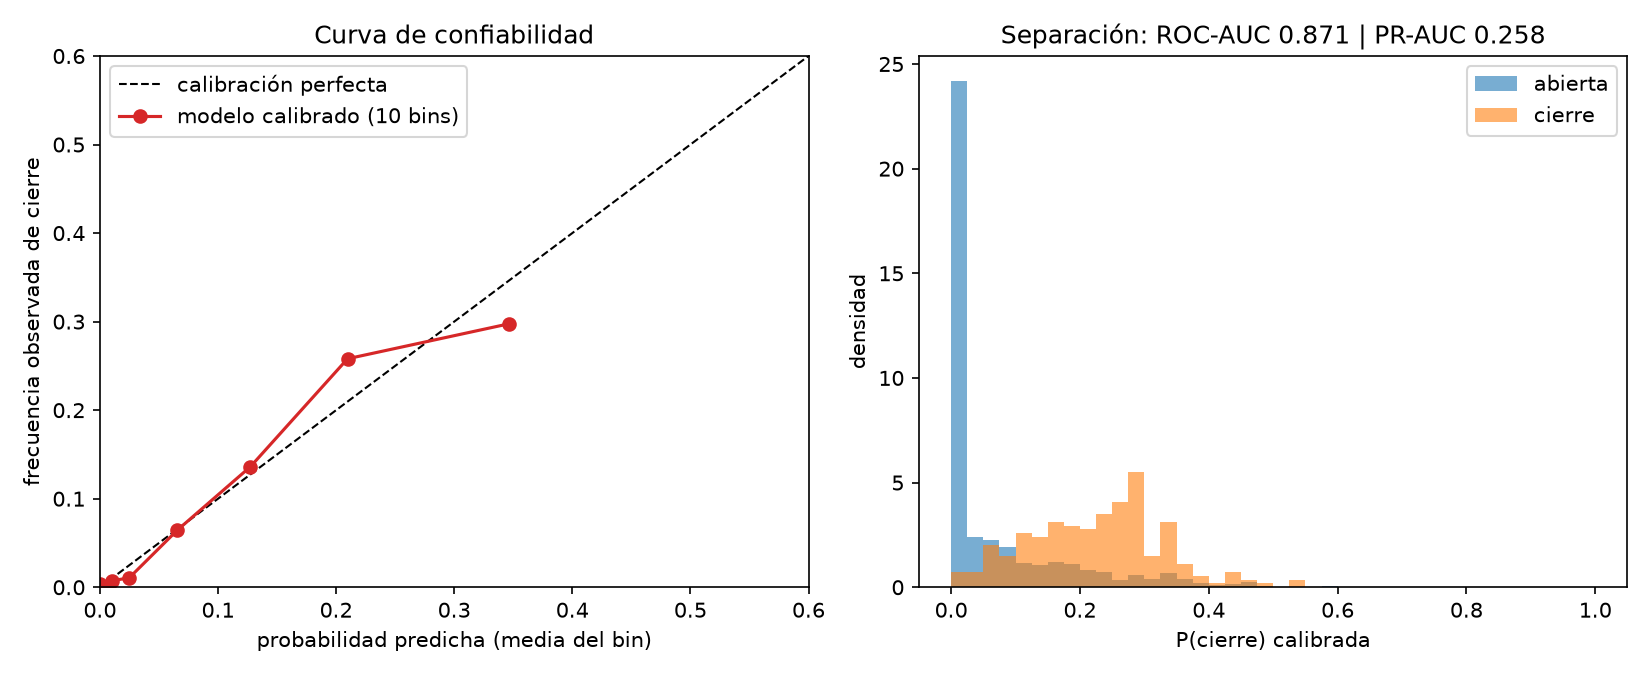
\includegraphics[width=0.92\textwidth]{../figures/fig03b_calibracion_logreg_all.png}
  \caption{Curva de confiabilidad tras la calibración y distribución de la probabilidad predicha
  para tramos abiertos y cerrados (regresión logística, bloque~A).}
  \label{fig:calibracion}
\end{figure}

\section{El mapa y para qué sirve}

Para cada tramo se guarda el puntaje predicho cuando ese tramo estuvo en el conjunto de prueba,
promediado sobre las diez semillas, junto con el desacuerdo entre semillas
(figura~\ref{fig:mapa}). El mapa proviene de la regresión logística, el único modelo cuyas
probabilidades superan a la tasa base (hallazgo~5). Como ordenamiento es útil: el 10\,\% de tramos
con mayor probabilidad (279) contiene 83 de los 217 cierres, es decir, el 38\,\%, 3,8 veces lo que
daría un orden al azar.

\begin{figure}[H]
  \centering
  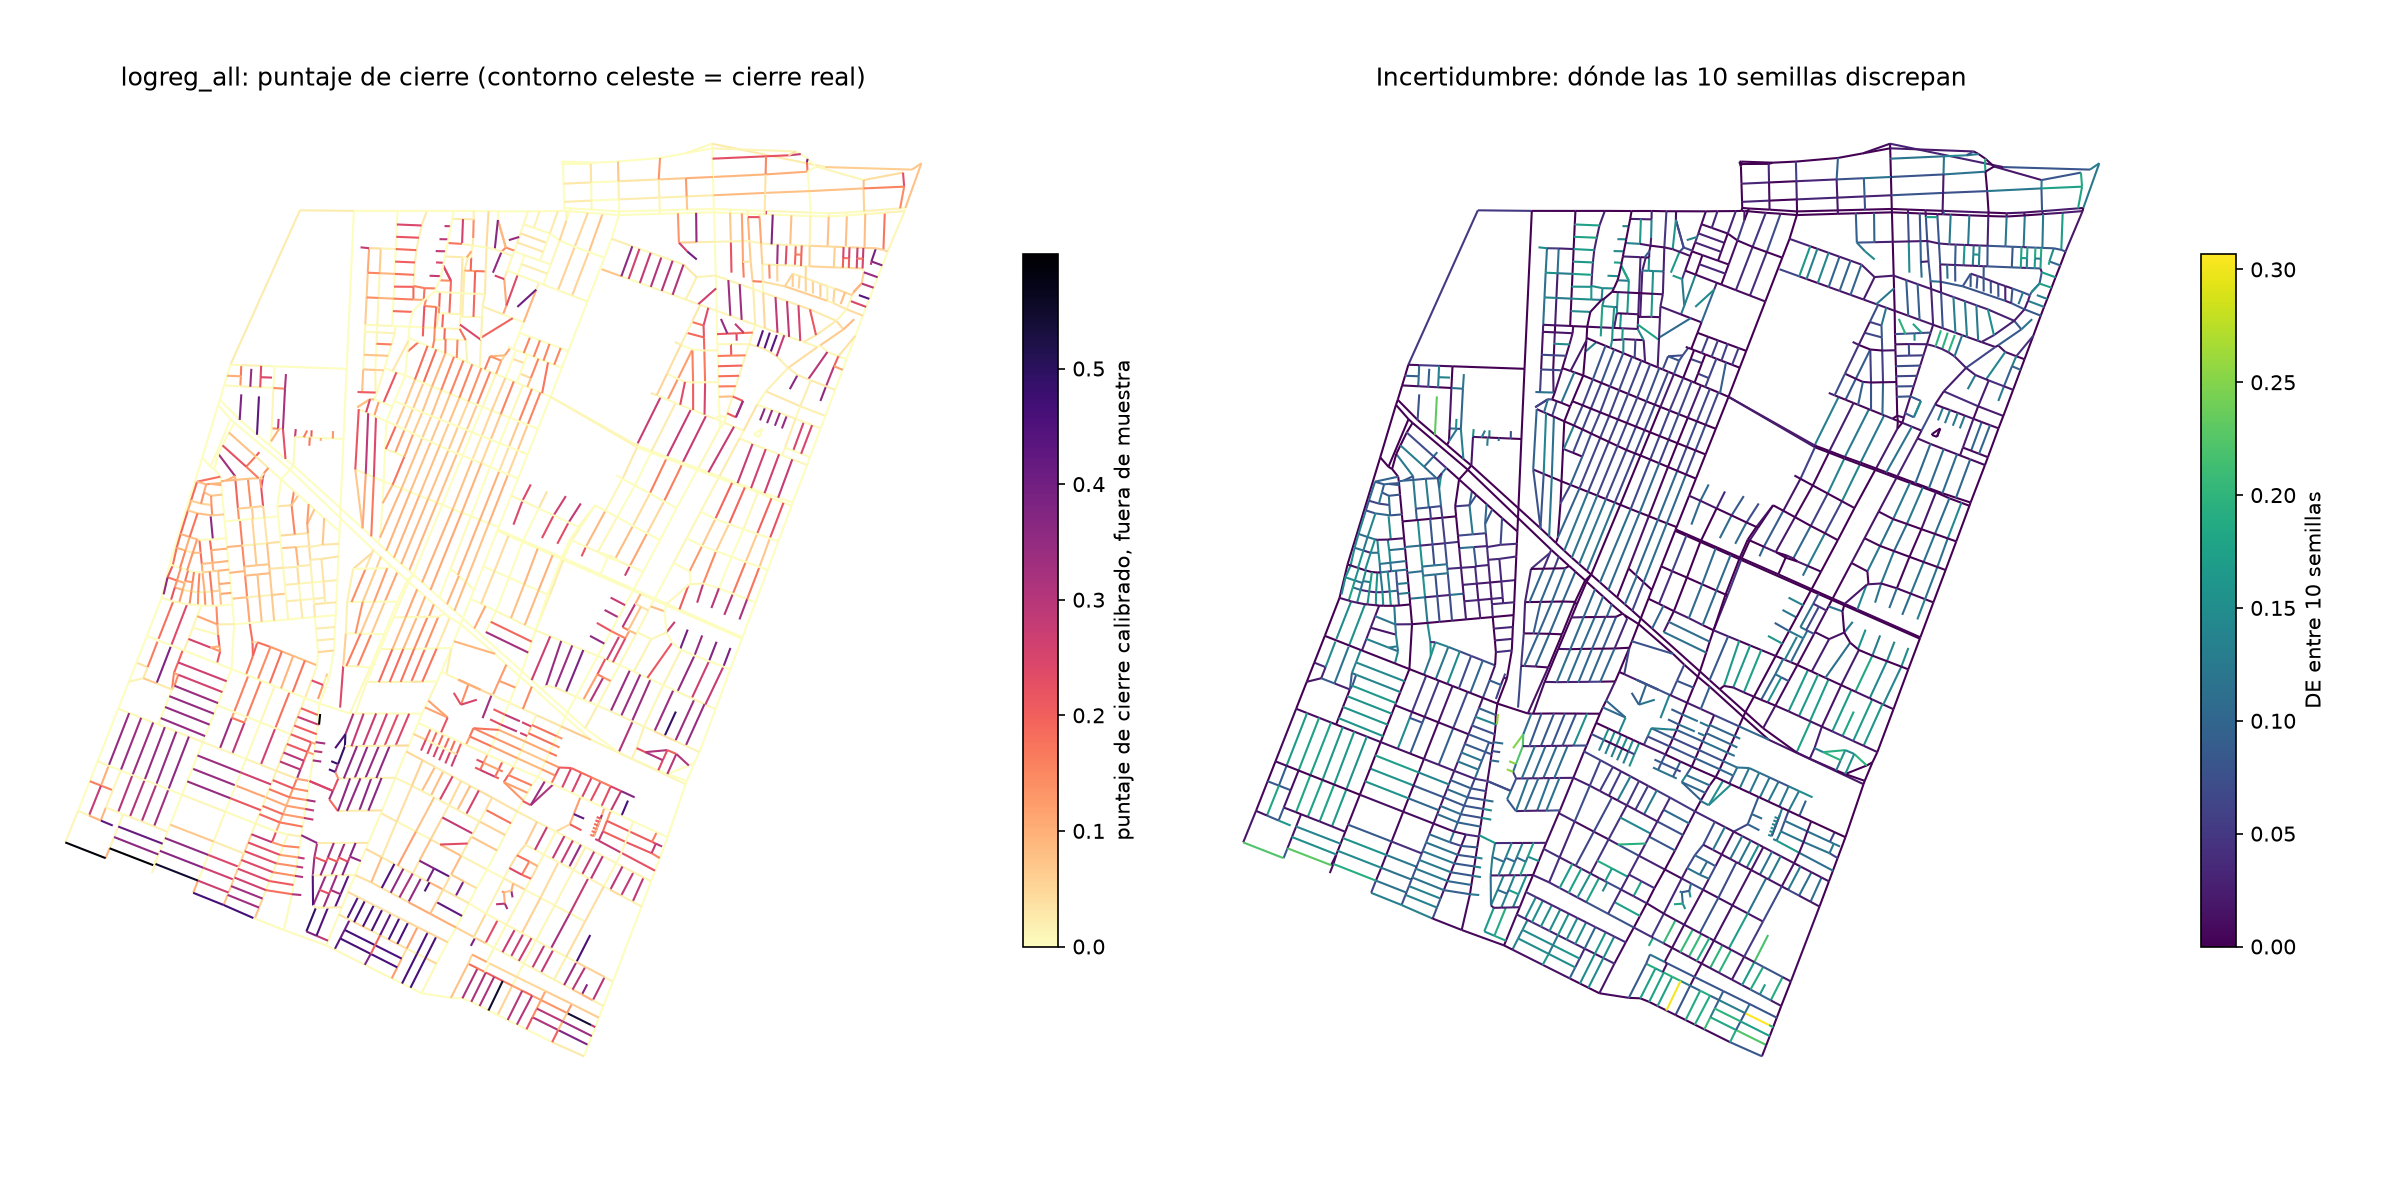
\includegraphics[width=\textwidth]{../figures/fig03a_mapa_logreg_all.png}
  \caption{Izquierda: probabilidad calibrada de cierre de cada tramo, predicha para barrios que el
  modelo no vio (regresión logística, bloque~A). Derecha: desacuerdo entre diez semillas.}
  \label{fig:mapa}
\end{figure}

La lectura más útil es la lista de \textbf{tramos abiertos que el modelo considera candidatos a
cierre} (figura~\ref{fig:candidatos}). Los primeros son pasajes y senderos como Pasaje 6 Norte,
Pasaje 1, Huafo, Anaxágoras, Tongoy y Paseo Grohnert ($p \approx 0{,}47$--$0{,}60$); algunos
senderos sin nombre deben verificarse en terreno, porque podrían no ser pasajes cerrables. Hay 207
tramos abiertos con $p \geq 0{,}25$, frente a 96 de los 217 cierres reales. Son hipótesis que un levantamiento futuro
puede confirmar o refutar; como el modelo ordena en lugar de predecir tramo a tramo, la lista es
una priorización para el trabajo de campo, no un pronóstico.

\begin{figure}[H]
  \centering
  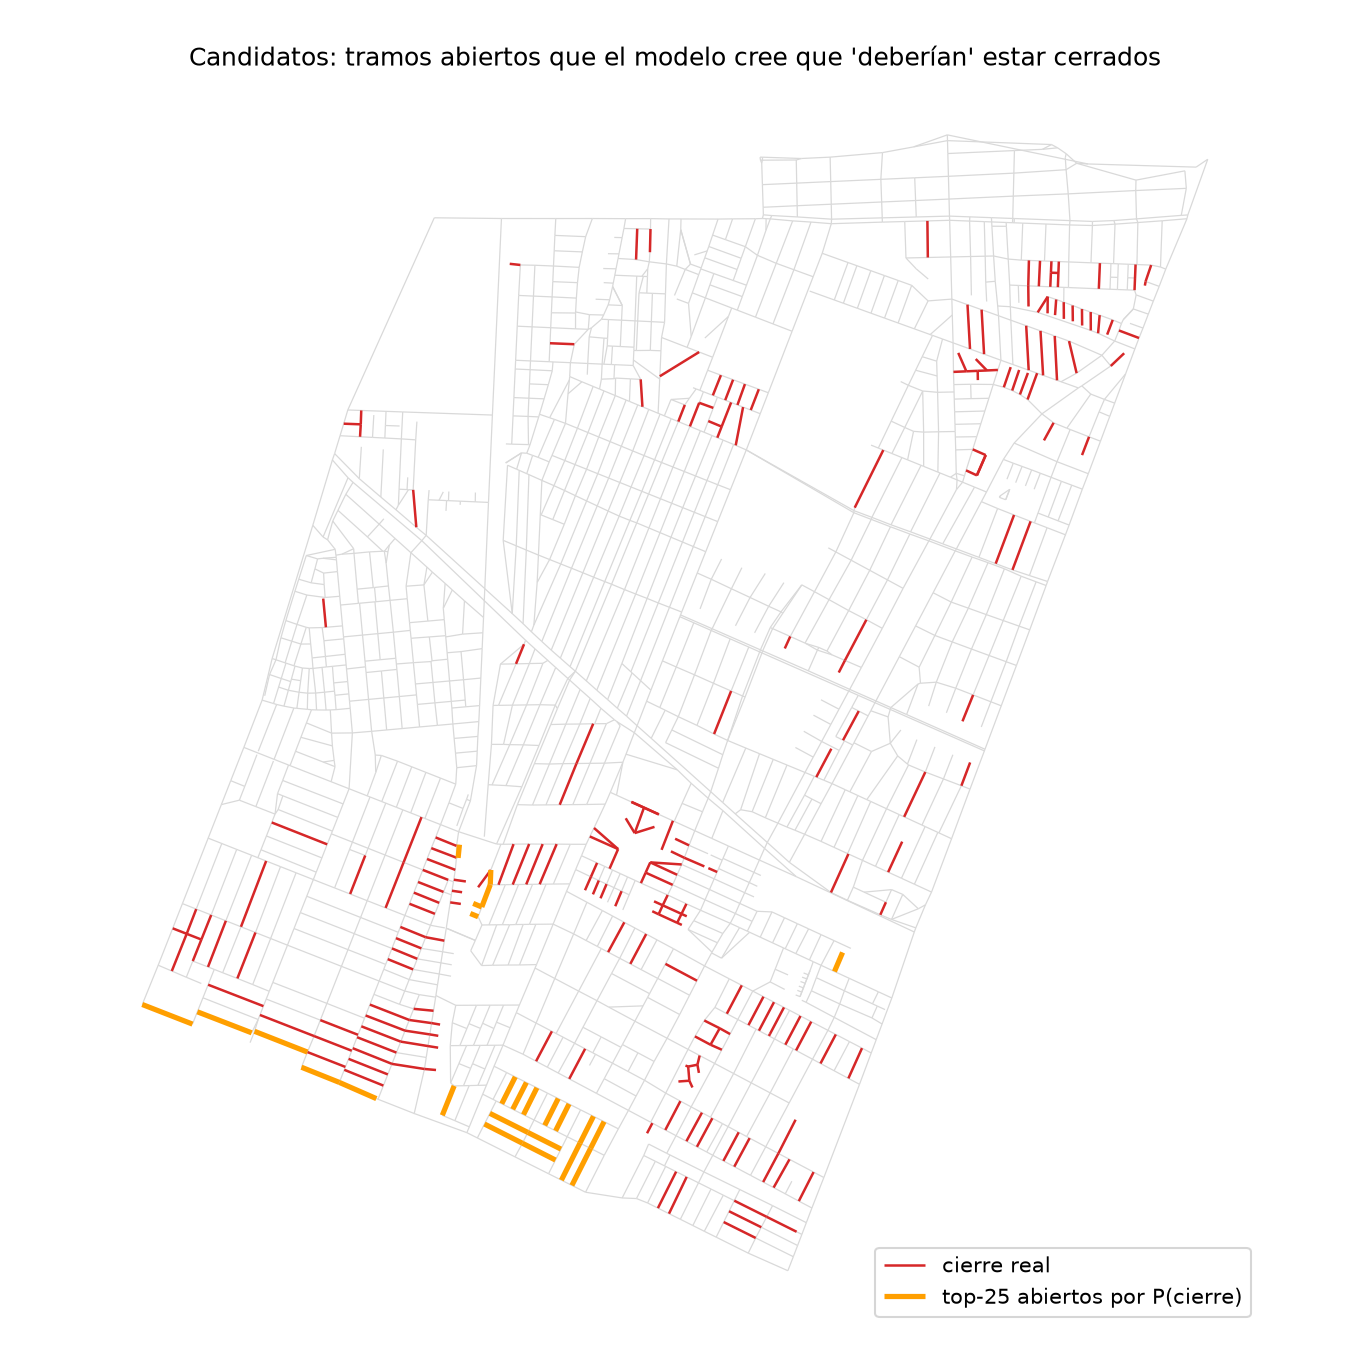
\includegraphics[width=0.6\textwidth]{../figures/fig03c_candidatos_logreg_all.png}
  \caption{Tramos abiertos con la mayor probabilidad de cierre según la regresión logística, sobre los cierres reales.}
  \label{fig:candidatos}
\end{figure}

\section{Replicación del estudio original}

Antes de construir nada nuevo se volvió a ejecutar el código del trabajo exploratorio previo desde los archivos
crudos. Sus dos enfoques se reproducen \textbf{exactamente}: los exponentes de densidad, el exceso
de 9 veces en la correlación de pares a unos 40\,m, las 18 celdas candidatas, las 23 neuronas
«calientes» del SOM, los 94 bloques candidatos, la asignación bloque a bloque, los perfiles de
conglomerado y los coeficientes de regresión. La auditoría dejó dos advertencias: el exponente
«fractal» de largo alcance es mayormente un efecto de tamaño finito (tres cuartos de la pendiente
aparecen en un modelo nulo con la misma geometría de red), y los conglomerados del SOM y sus
interpretaciones dependen de una sola semilla aleatoria (entre el 17 y el 19\,\% de los bloques
cambia de estado con otras semillas).

\section{Limitaciones y trabajo futuro}
\label{sec:limites}

\begin{itemize}[leftmargin=*]
  \item \textbf{Fechas de registro.} \codigo{año} es el año de registro del cierre, no
    necesariamente el de su construcción. El hallazgo~6 muestra que ambas cohortes comparten un
    patrón, pero no elimina el desfase temporal con las covariables del bloque~B.
  \item \textbf{Ubicación.} Una parte relevante de la señal proviene de la distancia al centroide,
    que es un indicador de ubicación y no de morfología.
  \item \textbf{Hiperparámetros.} Las arquitecturas neuronales se entrenaron con una receta común
    sin ajuste; un ajuste por arquitectura podría cambiar la comparación entre ellas, aunque es
    improbable que cierre la brecha con la regresión logística.
  \item \textbf{Geometría simplificada.} Los tramos se representan como rectas entre sus extremos;
    las polilíneas reales refinarían largos y mapas.
  \item \textbf{Condominios.} Los portones de condominio se tratan como «no cerrados» para mantener
    la definición del estudio original.
  \item \textbf{Próximos pasos.} Transferencia inductiva a La Florida y levantamiento de
    verificación de los 207 candidatos.
\end{itemize}

\section{Reproducibilidad}

Todo el código, los datos del levantamiento y las covariables están versionados en el repositorio.
Basta CPU; la batería completa tarda entre 20 y 40 minutos en un computador portátil.

\begin{verbatim}
git clone https://github.com/gdosramos/rejas-gnn.git && cd rejas-gnn
python -m pip install torch --index-url https://download.pytorch.org/whl/cpu
python -m pip install -r requirements-lock.txt
python -m pip install -e ".[dev]" --no-deps
python -m pytest        # 42 pruebas
make baselines          # líneas base no neuronales
make run-all            # ablación A/B x modelos x semillas 42-51
make paired             # comparaciones pareadas con IC
make cohorts            # análisis por cohorte de registro
\end{verbatim}

Cada ejecución guarda su configuración, las versiones de las bibliotecas y las métricas en JSON.
Dentro de una misma máquina, los resultados son reproducibles bit a bit. Entre máquinas (Linux x86
y Apple M1, ambas documentadas en el repositorio), las métricas de ordenamiento coinciden hasta el
tercer decimal.

\begin{thebibliography}{99}
\bibitem{brier1950} Brier, G.~W. (1950). Verification of forecasts expressed in terms of
  probability. \emph{Monthly Weather Review}, 78(1), 1--3.
\bibitem{brody2022} Brody, S., Alon, U. y Yahav, E. (2022). How attentive are graph attention
  networks? \emph{International Conference on Learning Representations}.
\bibitem{fey2019} Fey, M. y Lenssen, J.~E. (2019). Fast graph representation learning with
  PyTorch Geometric. \emph{ICLR Workshop on Representation Learning on Graphs and Manifolds}.
\bibitem{hamilton2017} Hamilton, W.~L., Ying, R. y Leskovec, J. (2017). Inductive representation
  learning on large graphs. \emph{Advances in Neural Information Processing Systems}, 30.
\bibitem{kipf2017} Kipf, T.~N. y Welling, M. (2017). Semi-supervised classification with graph
  convolutional networks. \emph{International Conference on Learning Representations}.
\bibitem{ley20499} Ley N.º 20.499 (2011). Regula el cierre de calles y pasajes por motivos de
  seguridad ciudadana. Diario Oficial de la República de Chile, 8 de febrero de 2011.
\bibitem{ley21411} Ley N.º 21.411 (2022). Modifica la Ley N.º 18.695, Orgánica Constitucional de
  Municipalidades, en materia de cierre o instalación de medidas de control de acceso en calles,
  pasajes o conjuntos habitacionales. Diario Oficial de la República de Chile, 25 de enero de 2022.
\bibitem{roberts2017} Roberts, D.~R. et al. (2017). Cross-validation strategies for data with
  temporal, spatial, hierarchical, or phylogenetic structure. \emph{Ecography}, 40(8), 913--929.
\bibitem{saito2015} Saito, T. y Rehmsmeier, M. (2015). The precision-recall plot is more
  informative than the ROC plot when evaluating binary classifiers on imbalanced datasets.
  \emph{PLOS ONE}, 10(3), e0118432.
\bibitem{wilcoxon1945} Wilcoxon, F. (1945). Individual comparisons by ranking methods.
  \emph{Biometrics Bulletin}, 1(6), 80--83.
\end{thebibliography}

\end{document}
